\chapter{Higher-genus dessins and reproducible finite carriers}
\label{book:computations}
The companion separates three objects: an exact combinatorial dessin, a chosen visualization of its surface, and a finite operator model. Agreement of their dimensions is not an equivalence of categories. We give constructions for which these distinctions can be checked directly.

\section{A hyperelliptic family beyond the torus}
For odd $m\ge3$, let $C_m$ be the smooth compactification of
\[
 y^2=x^m-1,\qquad \beta=x^m:C_m\longrightarrow\mathbb P^1.
\]
The affine curve is smooth: simultaneous vanishing of $2y$ and $mx^{m-1}$ would force $x=y=0$, which does not lie on the curve in characteristic zero. Its double cover of the $x$-line branches over the $m$ roots of unity and infinity. Riemann--Hurwitz gives $g=(m-1)/2$.

\begin{proposition}[Clean passports and infinite orders]
The degree-$2m$ Belyi map $\beta$ has passport
\[
 (m,m),\quad (2,\ldots,2)\ (m\text{ entries}),\quad (2m).
\]
Its contracted dessin has two vertices, $m$ edges and one face. With darts $0,\ldots,2m-1$, one may take
\[
 \sigma=(0\ 1\ \cdots\ m-1)(m\ m+1\ \cdots\ 2m-1),\quad
 \alpha=\prod_{j=0}^{m-1}(j\ j+m).
\]
The associated completed order has $k[[u]]$-rank $2m^2$, and the polynomial locally gentle algebra is infinite dimensional.
\end{proposition}
\begin{proof}
Over zero, $x$ is a local coordinate at the two points $y=\pm i$, and $x^m$ has index $m$. At a root $\xi$ of unity, $y$ is a local coordinate and $\beta-1=y^2$, giving index two. At the unique point at infinity, $x$ has pole order two, so $\beta$ has pole order $2m$. Away from these points, differentiating $x^m$ introduces no further branching. This proves the passport and the Belyi property. The two cycles describe the two lifts of the radial segments in the $x$-plane. The involution exchanges their lifts at the clean branch points. For odd $m$, $\phi=\alpha\sigma^{-1}$ is a single $2m$-cycle: its square advances two steps in each $m$-cycle, and two is invertible modulo $m$. Hence $2-2g=2-m+1$. Each permitted $m$-cycle repeats without meeting a forbidden pair. This proves infinite dimension; the earlier split-order theorem gives rank $m^2+m^2$.
\end{proof}
For $m=5$ this gives genus two and order rank fifty; for $m=7$ genus three and rank ninety-eight. These are actual cellular dessins, not finite-dimensional stand-ins. The all-degree resolutions are obtained by iterating their forbidden successor permutation, as in the general resolution theorem. The number of vertices of the algebra is $m$, while its coefficient-order rank is $2m^2$; they should not be interchanged in a quantum register count.

\begin{figure}[ht]\centering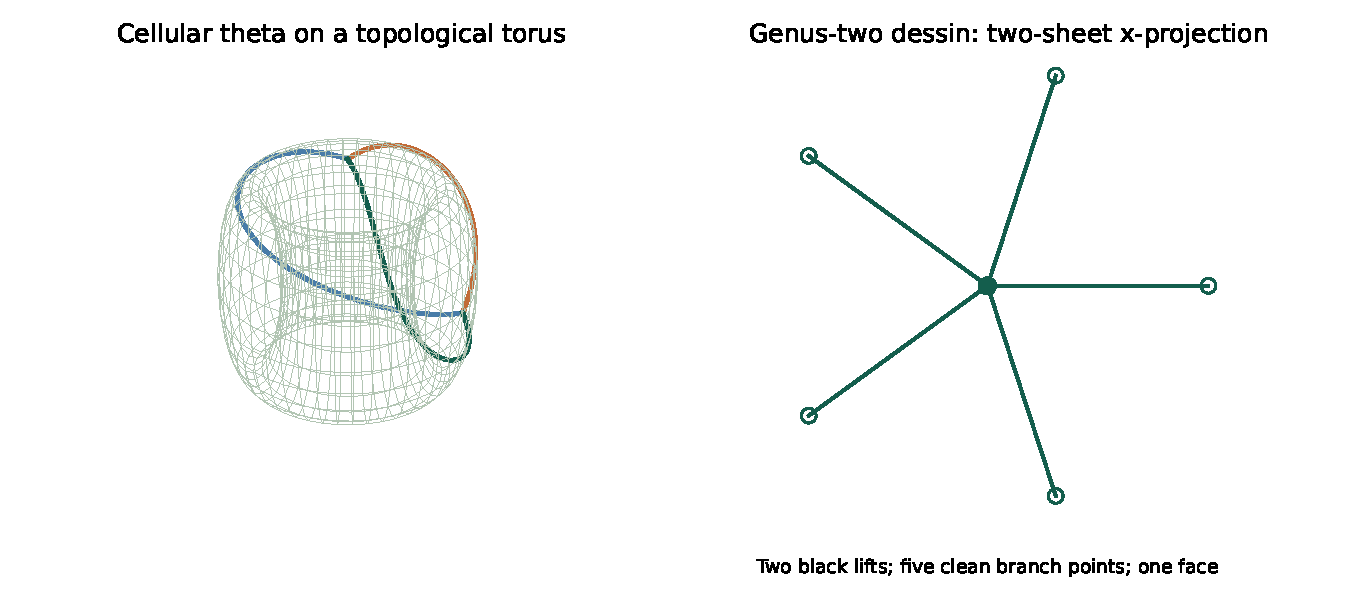
\includegraphics[width=\textwidth]{figures/dessin-carriers.pdf}
\caption{Two distinct kinds of faithful data display. Left: a topological torus embedding with the three periodic lifts of the theta graph. Right: the genus-two dessin's $x$-projection; every radial segment has two lifts. The right-hand disk is not the genus-two surface itself.}\end{figure}

\section{Larger genera and infinite hyperbolic windows}
The same exact family gives genus five ($m=11$, rank242), genus nine ($m=19$, rank722) and genus sixteen ($m=33$, rank2178). These ranks refer to the infinite completed orders over $k[[u]]$, not finite vector-space dimensions. The browser includes these examples and a four-dimensional rotation control: write $(x,y)\in\C^2$ in real coordinates $(x_1,x_2,y_1,y_2)$, rotate the $(x_1,y_1)$ plane, then project to three coordinates. The omitted coordinate and projected intersections are explicitly identified. This is a view of the affine double-cover sheets, not a claimed injective embedding of a compact higher-genus surface.

A separate example is the infinite regular hyperbolic $\{7,3\}$ tiling. Its heptagons have angles $2\pi/3$, so the defect formula gives area $5\pi-7(2\pi/3)=\pi/3$ at curvature $-1$. For a regular $\{p,q\}$ tiling, its central polygon's Poincar\'e circumradius is
\[
 r=\sqrt{\frac{\cos(\pi/p+\pi/q)}{\cos(\pi/p-\pi/q)}}.
\]
To derive this, bisect the polygon into right triangles with acute angles $\pi/p$ and $\pi/q$. The hyperbolic right-triangle identity is $\cosh R=\cot(\pi/p)\cot(\pi/q)$, while the disk radius is $r=\tanh(R/2)$. Substituting and applying elementary sum-to-product identities gives the formula. The condition $1/p+1/q<1/2$ ensures positive real radius.

A side is an arc of a circle with center $c$ and squared radius $|c|^2-1$, orthogonal to the unit disk. Its endpoints $a,b$ determine $\operatorname{Re}(a\bar c)=(|a|^2+1)/2$ and the analogous equation for $b$. Circle inversion gives its hyperbolic reflection
\[
 z\longmapsto c+\frac{|c|^2-1}{\bar z-\bar c}.
\]
If a side is a diameter, the circle formula is replaced by reflection in the line through the origin; the implementation handles that case separately. Reflecting adjacent polygons constructs finite windows of the infinite tiling. The implementation caps both depth and tile count and reports those bounds. It never calls a truncated window the whole infinite lattice. An optional Lorentz-hyperboloid view maps $z$ to $(2\operatorname{Re}z,2\operatorname{Im}z,1+|z|^2)/(1-|z|^2)$, satisfying $T^2-X^2-Y^2=1$. Its metric is Lorentzian ambient data, not the Euclidean metric of the rendered mesh. A finite compact surface quotient, its side pairings and an arithmetic correspondence would require separate certificates. The current lattice patch supplies none of them.

\section{What a three-dimensional view can claim}
The genus-one examples use a standard torus parameterization
\[
 ((R+r\cos v)\cos u,(R+r\cos v)\sin u,r\sin v),\quad R>r>0.
\]
The theta paths lift from $(0,0)$ to $(1/3,1/3)$ with translation vectors $(0,0),(-1,0),(0,-1)$ in the universal covering plane. Their interiors are disjoint on the quotient, and their complement is a disk; the induced rotations at the two black vertices give the one-face theta dessin. The elliptic square uses the two fundamental loops. These are topological realizations; the induced Euclidean torus metric is not asserted to be the constant-curvature or uniformizing metric of the algebraic curve.

For $m\ge5$, the companion instead plots a three-real-coordinate projection of the two sheets of $y^2=x^m-1$. Branch cuts, changes of sheet and the compact point at infinity remain part of the mathematical construction. Projected sheets can meet. No injective embedding or numerical uniformization follows from a screen image. The Sage source gives exact passports, quivers, forbidden pairs and determinant calculations. The installed \texttt{sage} launcher on this machine points to a missing application, so those Sage scripts are supplied but have not been executed in Sage in this milestone. Exact stdlib Python checks independently verify the displayed permutations, genus and ramification counts.

\section{Finite clocks and cross-backend agreement}
For $d\ge2$, let $Ue_j=\zeta^j e_j$, $Ve_j=e_{j+1}$, with $\zeta=e^{2\pi i/d}$. Then
\[
 UV=\zeta VU,\quad U^d=V^d=I.
\]
Applying the two sides to $e_j$ proves the first identity, including the wraparound because $\zeta^d=1$. The discrete Fourier matrix prepares the uniform superposition. The executable comparison applies $F$, then $U$, then $V$, on a four-level carrier; its relative phases are nonconstant. Cirq, Qiskit and PennyLane statevectors are compared to the reference vector. Strawberry Fields realizes the same $U(4)$ matrices on the single-photon subspace of four optical modes and compares the entire density block, including its off-diagonal phases. Preparing a Fock state need not leave the simulator's internal representation marked pure, so reading only a ket would be incorrect.

The photonic cutoff two is exact for this passive, single-photon computation: photon number is preserved and no mode ever contains more than one photon. This justification does not extend to arbitrary squeezing or multiphoton simulations. Separate NVIDIA cuQuantum and CUDA-Q adapters and pinned upstream forks are provided. GPU execution is not performed on this Mac; source availability is distinct from a successful accelerator run.

\chapter{Quantum feature models and auxiliary compression}
\label{book:learning}
These preserved experiments have distinct objectives. Local Ising regressors approximate selected coarse couplings but omit normalization and a full iterated action. QCNN compression, photonic principal-axis alignment and the Harper surrogate are auxiliary benchmarks. Actual partition-preserving RG and a trained full-action approximation are developed in Chapter~\ref{rg:chapter}. Here the exact targets, held-out samples, recorded seeds, classical optimizer and feature readouts are retained without calling these different objectives a complete RG flow.

\section{Exact teacher data from Ising decimation}
For spins $s_1,s_2,s_3\in\{-1,1\}$, summing the middle spin gives
\[
 \sum_{s_2}e^{K_1s_1s_2+K_2s_2s_3}
 =2\cosh(K_1s_1+K_2s_3)
 =A e^{K' s_1s_3},
\]
where
\[
 K'=\tfrac12\log\frac{\cosh(K_1+K_2)}{\cosh(K_1-K_2)}
 =\operatorname{arctanh}(\tanh K_1\tanh K_2),\quad
 A=2\sqrt{\cosh(K_1+K_2)\cosh(K_1-K_2)}.
\]
Checking $s_1s_3=\pm1$ proves the identities. Thus the normalization and coupling have separate roles. The network below learns $K'$, not the full partition-function normalization $A$.

For a three-valent star, let $s=(s_1,s_2,s_3)$ be boundary spins and sum its center. The exact boundary logarithmic weight is
\[
 f_K(s)=\log\bigl(2\cosh(K_1s_1+K_2s_2+K_3s_3)\bigr).
\]
Fourier expansion on the Boolean cube is orthogonal for $2^{-3}\sum_s$. The symmetry $f_K(-s)=f_K(s)$ removes every odd monomial. Consequently
\[
 f_K(s)=c(K)+\sum_{i<j}J_{ij}(K)s_is_j,\quad
 J_{ij}=2^{-3}\sum_s f_K(s)s_is_j.
\]
This proves the zero-field star-to-triangle reduction and supplies exact labels. Such trivalent patches occur at the black vertices of the theta dessin. The associated Ising Hamiltonian is a finite model on that graph, not a faithful representation of its completed surface order.

\section{Shared quantum graph convolution}
The input patch $(K_1,K_2)$ is encoded by
$R_y(K_1)\otimes R_y(K_2)|00\rangle$. Two layers of local $R_y,R_z$ rotations, a CZ entangler after each layer, and a final CNOT define an eight-parameter circuit $Q_\theta$. The three features are
\[
 z_\theta(K)=\bigl(\langle Z_0\rangle,\langle Z_1\rangle,\langle Z_0Z_1\rangle\bigr).
\]
A shared affine head predicts $\widehat K'=w\cdot z_\theta+b$. Twelve trainable parameters include the four readout coefficients. Independent samples are drawn uniformly from $[0.05,1.7]^2$: ninety are used for training and thirty are held out. The loss is the mean-square error against exact decimation. The independent constant predictor is fitted only on training targets.

For a gate $e^{-itP/2}$, $P^2=I$, and a fixed state and observable, the expectation has the form $a+b\cos t+c\sin t$. Hence
\[
 \partial_t z=\tfrac12\bigl(z(t+\pi/2)-z(t-\pi/2)\bigr).
\]
Each gate parameter occurs once. The code differentiates the expectation features with this formula and then applies the classical chain rule to the squared loss and affine head. Applying parameter shift to the squared loss itself would generally give a wrong gradient. A central finite-difference check of the implemented full loss gradient is recorded.

\section{QCNN compression with a genuine pooling channel}
The four-site periodic transverse-field Ising Hamiltonian is
\[
 H(h)=-\sum_{(i,j)\in C_4}Z_iZ_j-h\sum_{i=0}^3X_i.
\]
We diagonalize its $16\times16$ Hermitian matrix at thirty-six fields in $[0.15,2.4]$, using the normalized lowest eigenvectors as input states. Every fourth field, starting at index zero, is held out. The circuit has two shared-layout local rotation layers with CZ edges on $C_4$, followed by CNOTs $(0,2)$ and $(1,3)$. Its sixteen parameters are optimized to minimize
\[
 \mathcal L(\theta)=1-\frac1{N_{\rm train}}\sum_j
 \langle\psi_j|Q_\theta^*(I_{01}\otimes|00\rangle\langle00|_{23})Q_\theta|\psi_j\rangle.
\]
The output on retained qubits is
\[
 \mathcal E_\theta(\rho)=\operatorname{Tr}_{23}(Q_\theta\rho Q_\theta^*).
\]
Its Kraus maps are $K_b=(I\otimes\langle b|)Q_\theta$, so
$\sum_bK_b^*K_b=I$. Thus it is completely positive and trace preserving. For $\rho\ge0$ and any $v$, each summand $v^*K_b\rho K_b^*v$ is nonnegative; cyclicity of the finite trace proves trace preservation. The Lean interface verifies the finite-matrix positivity and trace statements with explicit completeness hypotheses. It does not formalize the optimizer or claim convergence of an infinite renormalization flow.

The compression loss is the weight discarded by the chosen vacuum projection. Its successful decrease measures improved concentration for this finite input family. It does not imply exact recovery of arbitrary four-qubit states, an isometry from dimension sixteen to four, or a critical fixed-point construction. The held-out loss remains appreciable, and is reported without calling the model lossless.

\section{A larger genus-four nine-qubit example}
The $m=9$ hyperelliptic dessin has genus four and completed-order rank162. Its nine edge labels index a permitted quiver cycle. A separate finite transverse-field Ising model is placed on this nine-cycle, with Hilbert-space dimension512. This uses the dessin's combinatorics, without claiming a faithful representation of its infinite order.

The larger experiment uses twelve ground states over fields $h\in[0.2,1.9]$, with nine training and three held-out states. These are numerical lowest-eigenstate approximations. The residual alone is not a rigorous lowest-energy certificate. A sparse Hermitian eigensolver has maximum recorded eigenpair residual $1.32\times10^{-13}$. The circuit has two layers of local $R_y,R_z$ gates and nearest-neighbor CZ around the cycle, with thirty-six parameters. Four CNOTs connect retained to discarded qubits, and tracing out four leaves a five-qubit output. Actual PennyLane gate simulation and parameter-shift gradients train for fifty updates. Final training and held-out discard losses are approximately $0.548$ and $0.409$. These substantial residuals are reported: this architecture is not an accurate lossless coarse graining. It is a reproducible larger testbed, with saved parameters, held-out examples and numerical ground-state residuals. The local page permits comparison with the smaller four-qubit model, while retaining their different data families and capacities.

\section{Quantum-feature graph attention}
Three two-qubit patch encoders use the same eight circuit parameters on the three pairs of the Ising star. Let their features be $z_e\in\R^3$. A learned query $q$ defines
\[
 \alpha_e=\frac{e^{q\cdot z_e}}{\sum_f e^{q\cdot z_f}},\quad
 c=\sum_e\alpha_e z_e,\qquad
 \widehat J_e=w_{\rm local}\cdot z_e+w_{\rm context}\cdot c+b.
\]
There are eighteen trainable parameters. One hundred star couplings are sampled from $[0.1,1.5]^3$, with seventy-five training and twenty-five held-out examples. The objective compares the three predictions with the exact Boolean-Fourier couplings above. The nonlinear attention head is differentiated by central differences of the complete training objective. This experiment is quantum-feature attention with a classical softmax head; it is not a fully coherent attention algorithm. The scalar labels do not assert permutation equivariance under conventions the implementation has not checked.

\begin{center}
\begin{tikzpicture}[node distance=5mm, every node/.style={font=\small}, b/.style={draw,rounded corners,align=center,text width=32mm,minimum height=13mm}]
\node[b] (a) {Exact finite\\physics data};
\node[b,right=of a] (b) {Shared quantum\\patch circuits};
\node[b,right=of b] (c) {Classical head\\or attention};
\node[b,right=of c] (d) {Held-out loss\\and exact checks};
\draw[-{Latex}] (a)--(b);\draw[-{Latex}] (b)--(c);\draw[-{Latex}] (c)--(d);
\end{tikzpicture}
\end{center}

\section{Photonic Gaussian pooling}
The Strawberry Fields experiment prepares two modes with opposite real squeezing $r$ and $-r$, then applies a fixed unknown-to-the-optimizer beam splitter angle $\alpha=0.47$. A learned shared beam splitter $\theta$ is optimized on twelve of sixteen squeezing values in $[0.1,0.9]$, holding out every fourth value. With $\hbar=2$, the covariance convention is $(x_0,x_1,p_0,p_1)$. The objective is
\[
 \operatorname{Var}(x_0)+\operatorname{Var}(p_1)
 =2\left[e^{-2r}\cos^2(\alpha+\theta)+e^{2r}\sin^2(\alpha+\theta)\right].
\]
This follows by applying the real beam-splitter rotation to the diagonal covariance of the two squeezed modes. Since $r>0$, its minimum occurs at $\theta=-\alpha$ modulo $\pi$, with value $2e^{-2r}$. The code trains the angle with central-difference gradients and compares its result with this known optimum. Pooling subsequently discards a mode; the experiment itself optimizes principal axes before that discard. It is a Gaussian finite-mode surrogate, not a demonstration of an interacting field-theory RG flow.

\begin{figure}[ht]\centering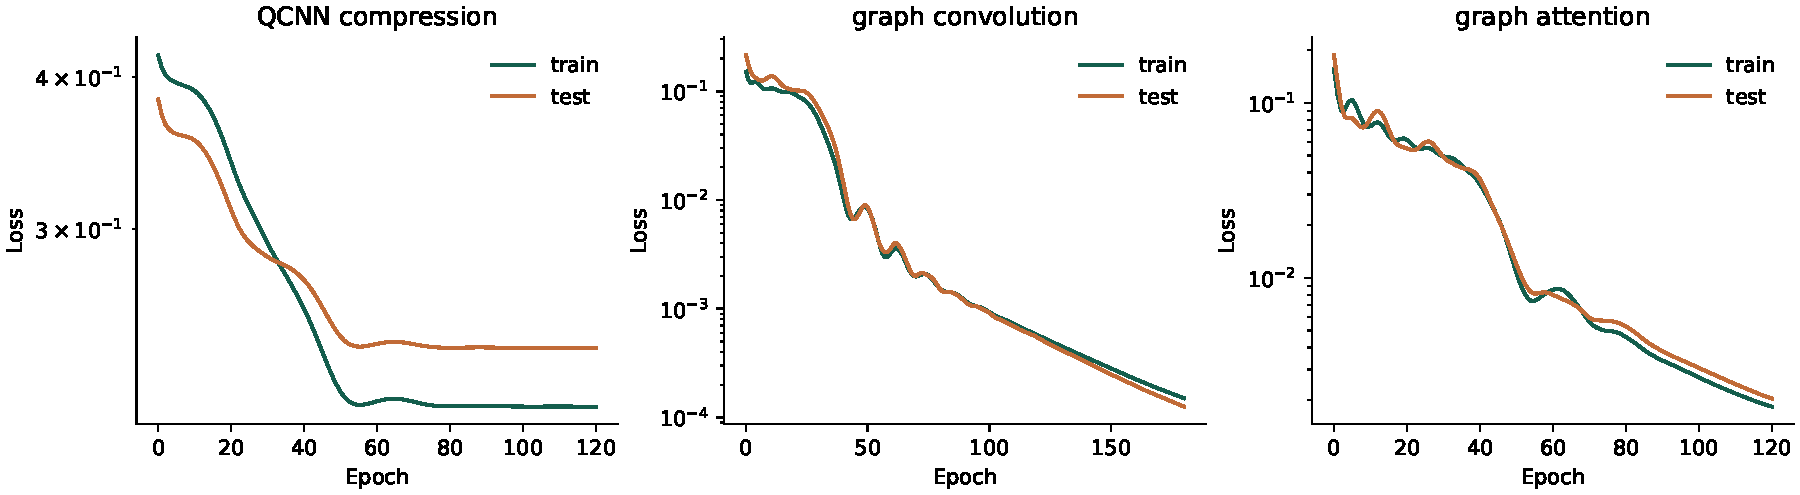
\includegraphics[width=\textwidth]{figures/training-curves.pdf}
\caption{Actual PennyLane CPU training runs, seed 20261103. Green is training loss; orange is held-out loss. Architectures have different objectives, so their vertical scales are not cross-model performance rankings.}\end{figure}
\begin{figure}[ht]\centering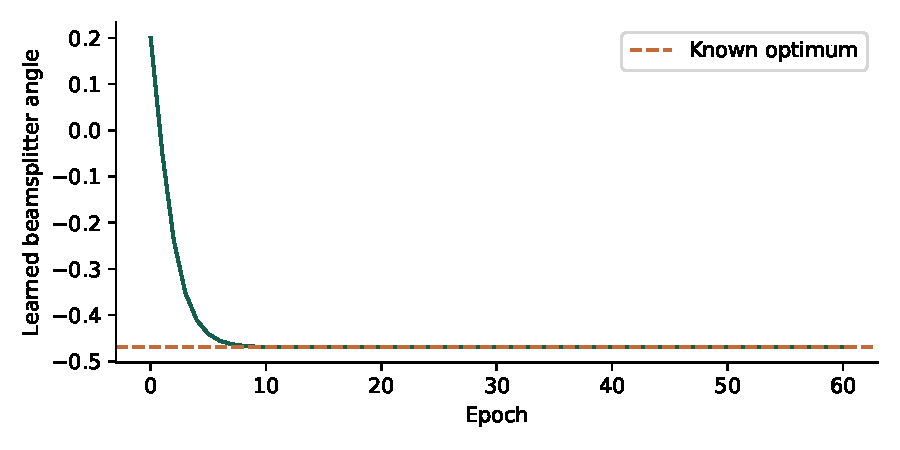
\includegraphics[width=.7\textwidth]{figures/photonic-angle.pdf}
\caption{Actual Strawberry Fields Gaussian simulation: the learned principal-axis angle approaches its independently known optimum.}\end{figure}
\begin{center}\small
\begin{tabular}{lrr}\toprule
Model & Initial held-out loss & Final held-out loss\\\midrule
Four-qubit QCNN compression & 0.38332 & 0.239725\\
Shared quantum graph convolution & 0.213652 & 0.000125897\\
Quantum-feature graph attention & 0.187065 & 0.00204477\\
\bottomrule\end{tabular}\end{center}


\section{Reproduction and limits of the evidence}
The scripts in \texttt{examples/quantum} specify each circuit, data generator, random seed and optimizer. The approved isolated environment is recorded in \texttt{requirements-cpu.lock}; existing environments and all pinned Lean toolchains remain unchanged. NumPy reference and actual PennyLane runs are saved separately. Cross-framework tests exercise a nontrivial Fourier/clock/shift state, not just a vacuum on which every diagonal clock is invisible. The Strawberry Fields run uses its Gaussian backend for training and its Fock backend for the separate one-photon comparison.

The companion's checkpoint slider selects a saved loss checkpoint. Its held-out examples use final weights; no intermediate predictions are implied. There are no hardware shots, cloud jobs or accelerator benchmarks. The training/test splits are deterministic interpolation tests on small synthetic families, not out-of-distribution or broad physical-validity tests. A model can help rank a proposed construction; it cannot discharge arithmetic holomorphy, determinant convergence, positivity or zero-location obligations merely by achieving low loss.
